\documentclass[tikz,border=8pt]{standalone}
\usepackage[T1]{fontenc}
\usepackage{helvet}
\renewcommand{\familydefault}{\sfdefault}
\usetikzlibrary{arrows.meta}

\definecolor{queryfill}{HTML}{DFF7F3}
\definecolor{queryborder}{HTML}{1BA99C}
\definecolor{corpusfill}{HTML}{FFF4D6}
\definecolor{corpusborder}{HTML}{D9A441}
\definecolor{bm25fill}{HTML}{FFE9C8}
\definecolor{bm25border}{HTML}{D88922}
\definecolor{nodefill}{HTML}{E8F2FF}
\definecolor{nodeborder}{HTML}{4E8CD8}
\definecolor{outfill}{HTML}{E7F6E7}
\definecolor{outborder}{HTML}{4FA64F}
\definecolor{softgray}{HTML}{F4F7FB}
\definecolor{darkline}{HTML}{333333}

\tikzset{
  card/.style={rectangle, rounded corners=5pt, align=center, draw=darkline, line width=0.8pt, minimum height=0.95cm, font=\small},
  query/.style={card, fill=queryfill, draw=queryborder, minimum width=2.1cm},
  corpus/.style={card, fill=corpusfill, draw=corpusborder, minimum width=2.25cm},
  bm25/.style={card, fill=bm25fill, draw=bm25border, minimum width=2.75cm},
  artifact/.style={card, fill=white, minimum width=2.75cm},
  output/.style={card, fill=outfill, draw=outborder, minimum width=2.75cm},
  softbox/.style={rectangle, rounded corners=8pt, draw=darkline, fill=softgray, line width=0.7pt},
  doc/.style={rectangle, rounded corners=3pt, fill=corpusfill, draw=corpusborder, line width=0.7pt, minimum width=0.46cm, minimum height=0.6cm},
  node/.style={circle, fill=nodefill, draw=nodeborder, line width=0.7pt, minimum size=0.30cm},
  finalnode/.style={circle, fill=outfill, draw=outborder, line width=0.7pt, minimum size=0.30cm},
  phase/.style={font=\small\bfseries, align=center},
  caption/.style={font=\scriptsize, align=center},
  flow/.style={-{Latex[length=2.2mm]}, line width=0.85pt, draw=darkline},
  faint/.style={dashed, darkline, opacity=0.30}
}

% Two flow rows keep every connector orthogonal.
\def\rtop{4.4}
\def\rbot{2.4}

\begin{document}
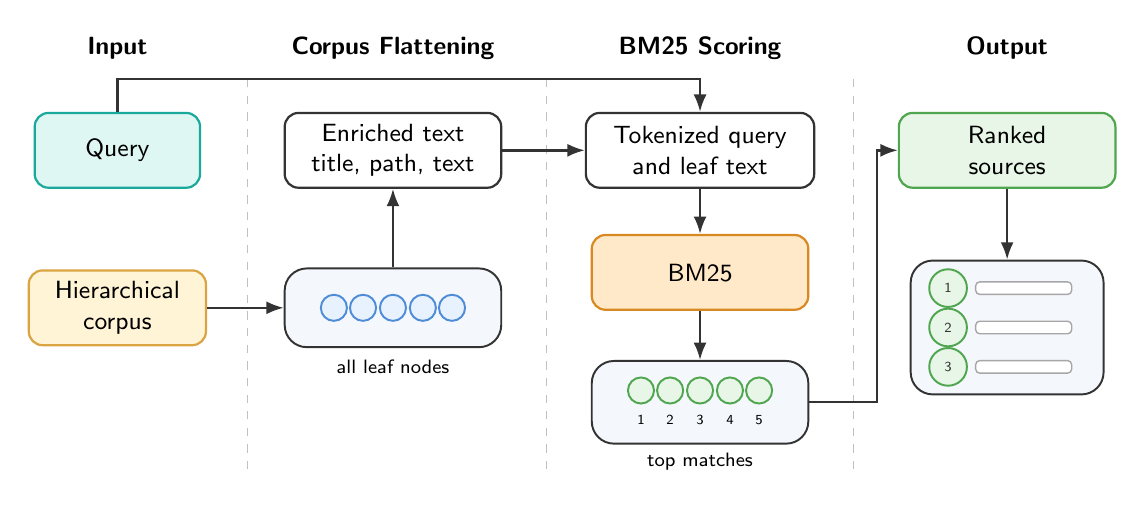
\begin{tikzpicture}

% Stage titles
\node[phase] at (1.5,5.7)  {Input};
\node[phase] at (5.0,5.7)  {Corpus Flattening};
\node[phase] at (8.9,5.7)  {BM25 Scoring};
\node[phase] at (12.8,5.7) {Output};

% Stage dividers
\draw[faint] (3.15,0.35)  -- (3.15,5.35);
\draw[faint] (6.95,0.35)  -- (6.95,5.35);
\draw[faint] (10.85,0.35) -- (10.85,5.35);

% --- Input ---
\node[query]  (query)  at (1.5,\rtop) {Query};
\node[corpus] (corpus) at (1.5,\rbot) {Hierarchical\\corpus};

% --- Corpus Flattening: collect all leaf nodes, then enrich each ---
\node[softbox, minimum width=2.75cm, minimum height=1.0cm] (allnodes) at (5.0,\rbot) {};
\foreach \x in {4.25,4.62,5.00,5.38,5.75} { \node[node] at (\x,\rbot) {}; }
\node[caption] at (5.0,1.65) {all leaf nodes};
\node[artifact] (enriched) at (5.0,\rtop) {Enriched text\\title, path, text};

% --- BM25 Scoring ---
\node[artifact, minimum width=2.9cm] (tokens) at (8.9,\rtop) {Tokenized query\\and leaf text};
\node[bm25]     (bm25)   at (8.9,2.85) {BM25};
\node[softbox, minimum width=2.75cm, minimum height=1.05cm] (ranked) at (8.9,1.2) {};
\foreach \x/\lab in {8.15/1,8.52/2,8.90/3,9.28/4,9.65/5} {
  \node[finalnode] at (\x,1.35) {};
  \node[font=\tiny] at (\x,0.98) {\lab};
}
\node[caption] at (8.9,0.45) {top matches};

% --- Output ---
\node[output] (sources) at (12.8,\rtop) {Ranked\\sources};
\node[softbox, minimum width=2.45cm, minimum height=1.7cm] (rankbox) at (12.8,2.15) {};
\foreach \y/\lab in {2.65/1,2.15/2,1.65/3} {
  \node[finalnode, minimum size=0.34cm, font=\tiny, text=darkline] at (12.05,\y) {\lab};
  \filldraw[rounded corners=1.5pt, fill=white, draw=black!35, line width=0.5pt]
    (12.40,\y-0.08) rectangle (13.62,\y+0.08);
}

% --- Flow ---
% Bottom row: corpus flattened into all leaf nodes (straight horizontal)
\draw[flow] (corpus.east) -- (allnodes.west);
% Flatten step up (enrich), then horizontal hand-off into scoring
\draw[flow] (allnodes.north) -- (enriched.south);
\draw[flow] (enriched.east)  -- (tokens.west);
% Query joins tokenization over the top
\draw[flow] (query.north) -- ++(0,0.42) -| (tokens.north);
% Scoring chain (vertical)
\draw[flow] (tokens.south) -- (bm25.north);
\draw[flow] (bm25.south)   -- (ranked.north);
% Top matches promoted to ranked output (right-angle riser)
\draw[flow] (ranked.east) -- (11.15,1.2) -- (11.15,\rtop) -- (sources.west);
\draw[flow] (sources.south) -- (rankbox.north);

\end{tikzpicture}
\end{document}
